% Options for packages loaded elsewhere
\PassOptionsToPackage{unicode}{hyperref}
\PassOptionsToPackage{hyphens}{url}
\PassOptionsToPackage{dvipsnames,svgnames,x11names}{xcolor}
%
\documentclass[
  letterpaper,
  DIV=11,
  numbers=noendperiod]{scrreprt}

\usepackage{amsmath,amssymb}
\usepackage{iftex}
\ifPDFTeX
  \usepackage[T1]{fontenc}
  \usepackage[utf8]{inputenc}
  \usepackage{textcomp} % provide euro and other symbols
\else % if luatex or xetex
  \usepackage{unicode-math}
  \defaultfontfeatures{Scale=MatchLowercase}
  \defaultfontfeatures[\rmfamily]{Ligatures=TeX,Scale=1}
\fi
\usepackage{lmodern}
\ifPDFTeX\else  
    % xetex/luatex font selection
\fi
% Use upquote if available, for straight quotes in verbatim environments
\IfFileExists{upquote.sty}{\usepackage{upquote}}{}
\IfFileExists{microtype.sty}{% use microtype if available
  \usepackage[]{microtype}
  \UseMicrotypeSet[protrusion]{basicmath} % disable protrusion for tt fonts
}{}
\makeatletter
\@ifundefined{KOMAClassName}{% if non-KOMA class
  \IfFileExists{parskip.sty}{%
    \usepackage{parskip}
  }{% else
    \setlength{\parindent}{0pt}
    \setlength{\parskip}{6pt plus 2pt minus 1pt}}
}{% if KOMA class
  \KOMAoptions{parskip=half}}
\makeatother
\usepackage{xcolor}
\setlength{\emergencystretch}{3em} % prevent overfull lines
\setcounter{secnumdepth}{5}
% Make \paragraph and \subparagraph free-standing
\ifx\paragraph\undefined\else
  \let\oldparagraph\paragraph
  \renewcommand{\paragraph}[1]{\oldparagraph{#1}\mbox{}}
\fi
\ifx\subparagraph\undefined\else
  \let\oldsubparagraph\subparagraph
  \renewcommand{\subparagraph}[1]{\oldsubparagraph{#1}\mbox{}}
\fi


\providecommand{\tightlist}{%
  \setlength{\itemsep}{0pt}\setlength{\parskip}{0pt}}\usepackage{longtable,booktabs,array}
\usepackage{calc} % for calculating minipage widths
% Correct order of tables after \paragraph or \subparagraph
\usepackage{etoolbox}
\makeatletter
\patchcmd\longtable{\par}{\if@noskipsec\mbox{}\fi\par}{}{}
\makeatother
% Allow footnotes in longtable head/foot
\IfFileExists{footnotehyper.sty}{\usepackage{footnotehyper}}{\usepackage{footnote}}
\makesavenoteenv{longtable}
\usepackage{graphicx}
\makeatletter
\def\maxwidth{\ifdim\Gin@nat@width>\linewidth\linewidth\else\Gin@nat@width\fi}
\def\maxheight{\ifdim\Gin@nat@height>\textheight\textheight\else\Gin@nat@height\fi}
\makeatother
% Scale images if necessary, so that they will not overflow the page
% margins by default, and it is still possible to overwrite the defaults
% using explicit options in \includegraphics[width, height, ...]{}
\setkeys{Gin}{width=\maxwidth,height=\maxheight,keepaspectratio}
% Set default figure placement to htbp
\makeatletter
\def\fps@figure{htbp}
\makeatother
\newlength{\cslhangindent}
\setlength{\cslhangindent}{1.5em}
\newlength{\csllabelwidth}
\setlength{\csllabelwidth}{3em}
\newlength{\cslentryspacingunit} % times entry-spacing
\setlength{\cslentryspacingunit}{\parskip}
\newenvironment{CSLReferences}[2] % #1 hanging-ident, #2 entry spacing
 {% don't indent paragraphs
  \setlength{\parindent}{0pt}
  % turn on hanging indent if param 1 is 1
  \ifodd #1
  \let\oldpar\par
  \def\par{\hangindent=\cslhangindent\oldpar}
  \fi
  % set entry spacing
  \setlength{\parskip}{#2\cslentryspacingunit}
 }%
 {}
\usepackage{calc}
\newcommand{\CSLBlock}[1]{#1\hfill\break}
\newcommand{\CSLLeftMargin}[1]{\parbox[t]{\csllabelwidth}{#1}}
\newcommand{\CSLRightInline}[1]{\parbox[t]{\linewidth - \csllabelwidth}{#1}\break}
\newcommand{\CSLIndent}[1]{\hspace{\cslhangindent}#1}

\KOMAoption{captions}{tableheading}
\makeatletter
\makeatother
\makeatletter
\@ifpackageloaded{bookmark}{}{\usepackage{bookmark}}
\makeatother
\makeatletter
\@ifpackageloaded{caption}{}{\usepackage{caption}}
\AtBeginDocument{%
\ifdefined\contentsname
  \renewcommand*\contentsname{Table of contents}
\else
  \newcommand\contentsname{Table of contents}
\fi
\ifdefined\listfigurename
  \renewcommand*\listfigurename{List of Figures}
\else
  \newcommand\listfigurename{List of Figures}
\fi
\ifdefined\listtablename
  \renewcommand*\listtablename{List of Tables}
\else
  \newcommand\listtablename{List of Tables}
\fi
\ifdefined\figurename
  \renewcommand*\figurename{Figure}
\else
  \newcommand\figurename{Figure}
\fi
\ifdefined\tablename
  \renewcommand*\tablename{Table}
\else
  \newcommand\tablename{Table}
\fi
}
\@ifpackageloaded{float}{}{\usepackage{float}}
\floatstyle{ruled}
\@ifundefined{c@chapter}{\newfloat{codelisting}{h}{lop}}{\newfloat{codelisting}{h}{lop}[chapter]}
\floatname{codelisting}{Listing}
\newcommand*\listoflistings{\listof{codelisting}{List of Listings}}
\makeatother
\makeatletter
\@ifpackageloaded{caption}{}{\usepackage{caption}}
\@ifpackageloaded{subcaption}{}{\usepackage{subcaption}}
\makeatother
\makeatletter
\@ifpackageloaded{tcolorbox}{}{\usepackage[skins,breakable]{tcolorbox}}
\makeatother
\makeatletter
\@ifundefined{shadecolor}{\definecolor{shadecolor}{rgb}{.97, .97, .97}}
\makeatother
\makeatletter
\makeatother
\makeatletter
\makeatother
\ifLuaTeX
  \usepackage{selnolig}  % disable illegal ligatures
\fi
\IfFileExists{bookmark.sty}{\usepackage{bookmark}}{\usepackage{hyperref}}
\IfFileExists{xurl.sty}{\usepackage{xurl}}{} % add URL line breaks if available
\urlstyle{same} % disable monospaced font for URLs
\hypersetup{
  pdftitle={Slum detection like a boss},
  pdfauthor={Shiraz Adamaly; Raya Berova; Thomas Faria; Clément Guillo; Judith Nabec; Tom Seimandi},
  colorlinks=true,
  linkcolor={blue},
  filecolor={Maroon},
  citecolor={Blue},
  urlcolor={Blue},
  pdfcreator={LaTeX via pandoc}}

\title{Slum detection like a boss}
\author{Shiraz Adamaly \and Raya Berova \and Thomas Faria \and Clément
Guillo \and Judith Nabec \and Tom Seimandi}
\date{2023-08-04}

\begin{document}
\maketitle
\ifdefined\Shaded\renewenvironment{Shaded}{\begin{tcolorbox}[interior hidden, boxrule=0pt, sharp corners, enhanced, frame hidden, borderline west={3pt}{0pt}{shadecolor}, breakable]}{\end{tcolorbox}}\fi

\renewcommand*\contentsname{Contents}
{
\hypersetup{linkcolor=}
\setcounter{tocdepth}{2}
\tableofcontents
}
\bookmarksetup{startatroot}

\hypertarget{project-description}{%
\chapter*{Project description}\label{project-description}}
\addcontentsline{toc}{chapter}{Project description}

\markboth{Project description}{Project description}

\bookmarksetup{startatroot}

\hypertarget{introduction}{%
\chapter{Introduction}\label{introduction}}

Je peux citer comme cela quelques articles que j'ai lu : Mboga et al.
(2017), Duque, Patino, and Betancourt (2017)\ldots{}

\begin{itemize}
\tightlist
\item
  Enquête cartographique réalisée chaque année dans les antilles
\item
  Coûteuse en termes de moyens humains
\item
  Apparition de zones d'habitations précaires possibles, dur de bien
  calibrer la charge d'enquête
\item
  On voudrait connaître chaque année les apparitions et disparition de
  logements même de courte durée !
\end{itemize}

\hypertarget{un-bidonville-le-mont-baduel}{%
\section{Un bidonville, le mont
Baduel}\label{un-bidonville-le-mont-baduel}}

\begin{figure}[H]

{\centering 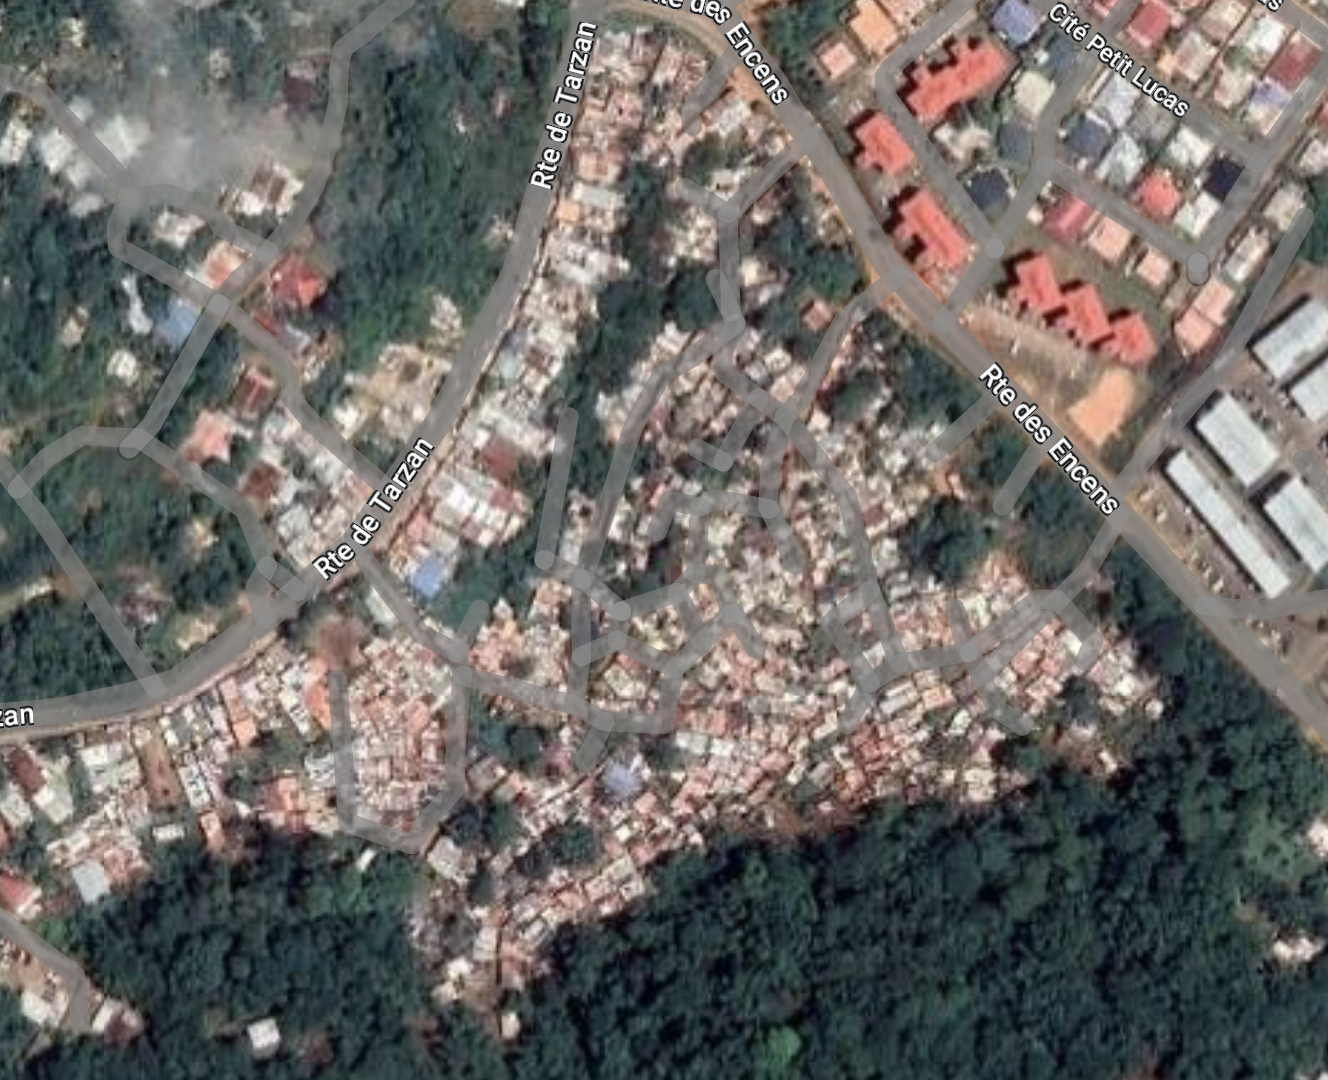
\includegraphics{figures/MontBaduel_2.png}

}

\caption{\label{fig-mont-baduel}Mont Baduel}

\end{figure}

\begin{figure}[H]

{\centering 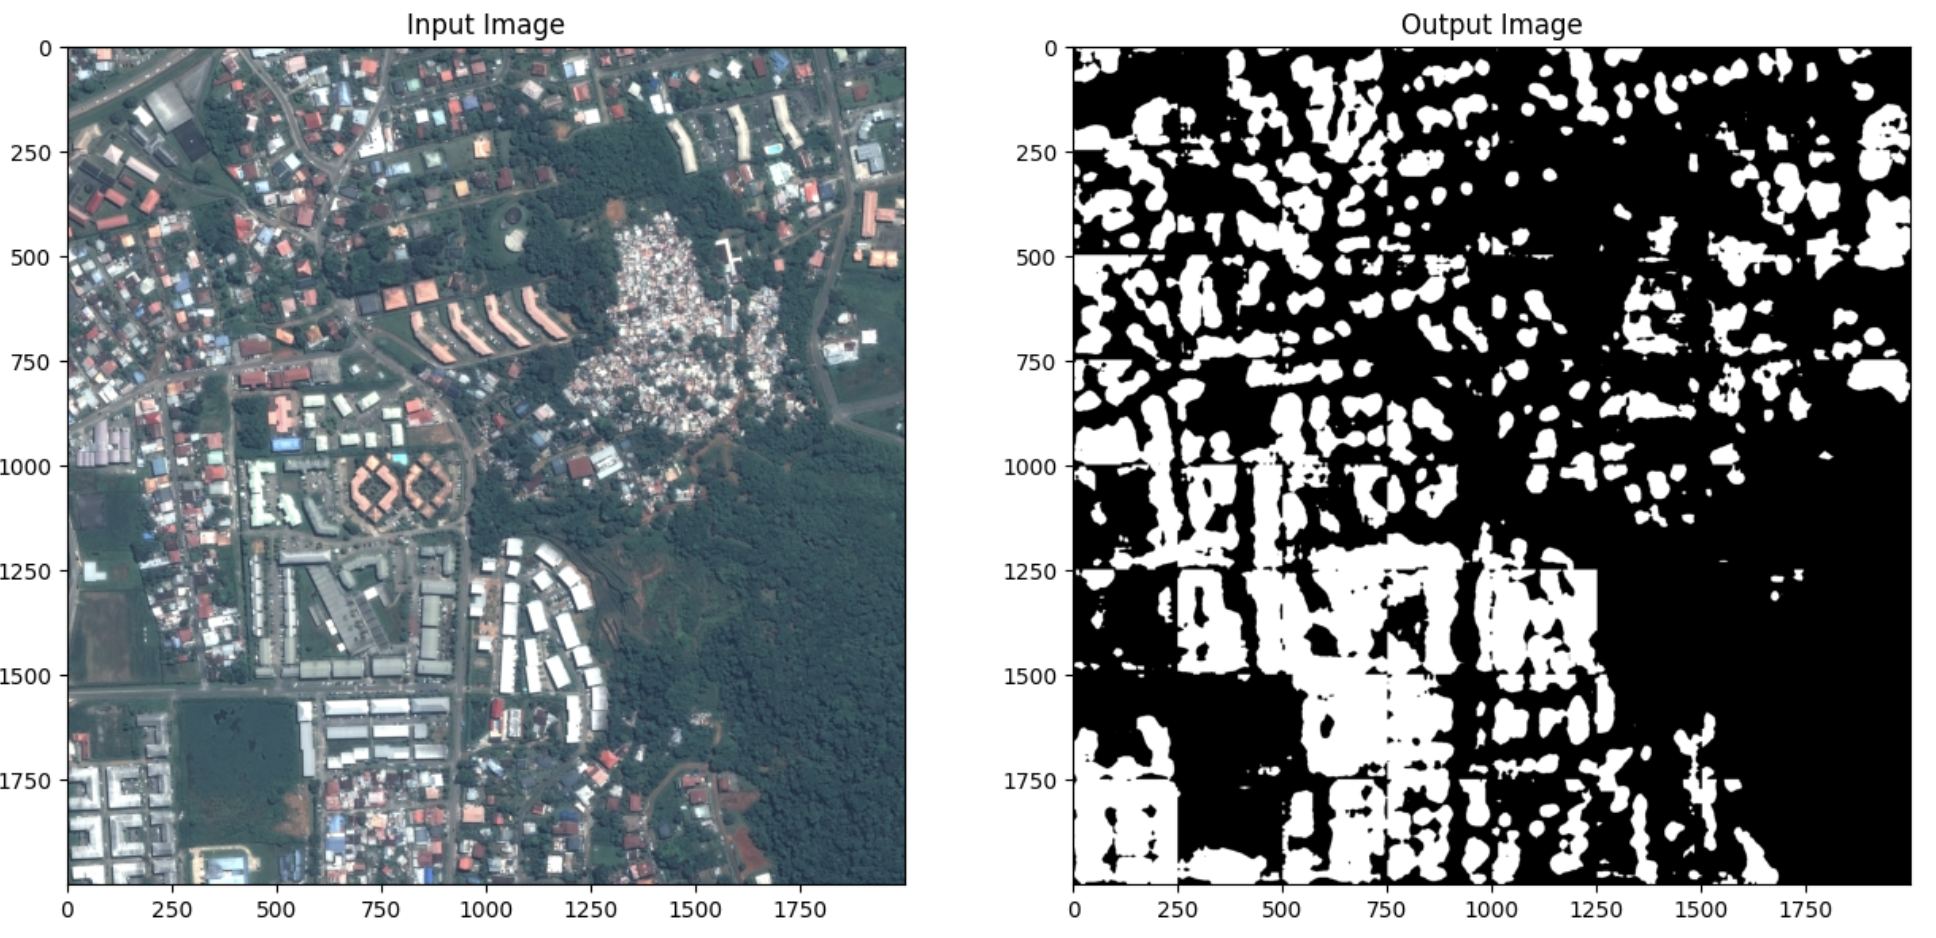
\includegraphics{figures/Detection_mont_baduel.png}

}

\caption{\label{fig-detec-mont-baduel}Détection du Mont Baduel}

\end{figure}

\begin{itemize}
\tightlist
\item
  On peut détecter la présence de bidonvilles !
\end{itemize}

\hypertarget{les-attendus-techniques-du-projet-sont-il-bien-duxe9finis}{%
\section{Les attendus techniques du projet sont-il bien définis
?}\label{les-attendus-techniques-du-projet-sont-il-bien-duxe9finis}}

\begin{itemize}
\tightlist
\item
  On voudrait ici être en mesure pour une zone donnée de détecter des
  apparitions ou disparitions de logement
\item
  A-t'on des données annotées qui nous permettent réellement de le faire
  ?
\end{itemize}

\bookmarksetup{startatroot}

\hypertarget{les-images-en-entruxe9es}{%
\chapter{Les images en entrées}\label{les-images-en-entruxe9es}}

\hypertarget{une-image-satellite}{%
\section{Une image satellite}\label{une-image-satellite}}

Plusieurs caractéristiques possibles pour une image satellite :

\begin{itemize}
\tightlist
\item
  \textbf{La résolution :} équivalence entre un pixel et le nombre de
  mètre couvert par ce dernier
\item
  \textbf{La fréquence d'acquisition :} fréquence des prises de vue pour
  un même endroit
\item
  \textbf{source de l'émission :} optique, radar, laser
\item
  \textbf{une fauchée :} Largeur de la zone enregistrée sur un passage
\item
  \textbf{Une couverture géographique donnée}
\end{itemize}

\hypertarget{images-faibles-ruxe9solution}{%
\section{Images Faibles résolution}\label{images-faibles-ruxe9solution}}

\begin{figure}[H]

{\centering 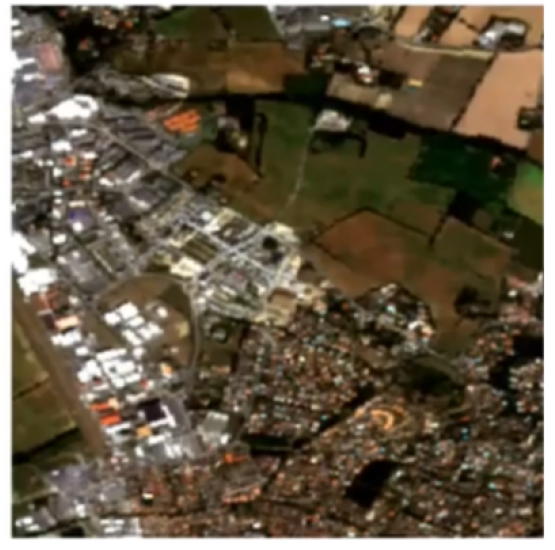
\includegraphics{figures/image_sentinel.png}

}

\caption{\label{fig-im-sentinel2}Images Sentinel 2, résolution : 10 m,
fréquence : tous les 5 jours, gratuites}

\end{figure}

\begin{figure}[H]

{\centering 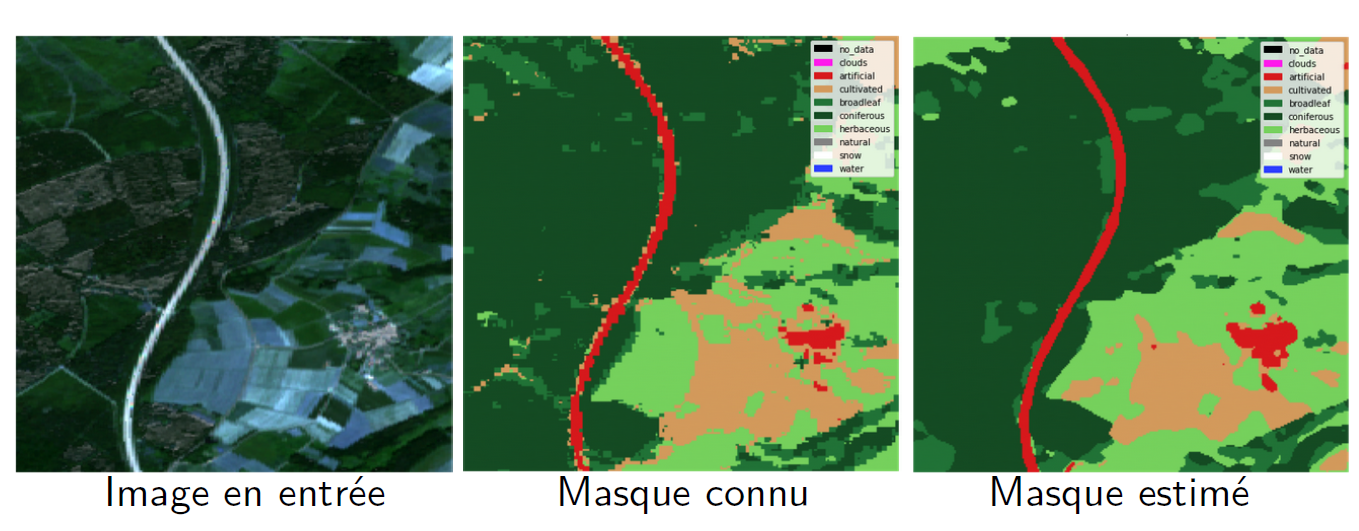
\includegraphics{figures/Exemple_1.png}

}

\caption{\label{fig-ex-sentinel2}Exemple masques Sentinel 2}

\end{figure}

\begin{itemize}
\tightlist
\item
  On ne peut espérer obtenir plus précis de ces images que ne peut
  permettre la résolution
\end{itemize}

\hypertarget{images-haute-ruxe9solution-les-donnuxe9es-pleiades}{%
\section{Images haute résolution : les données
pleiades}\label{images-haute-ruxe9solution-les-donnuxe9es-pleiades}}

\begin{figure}[H]

{\centering 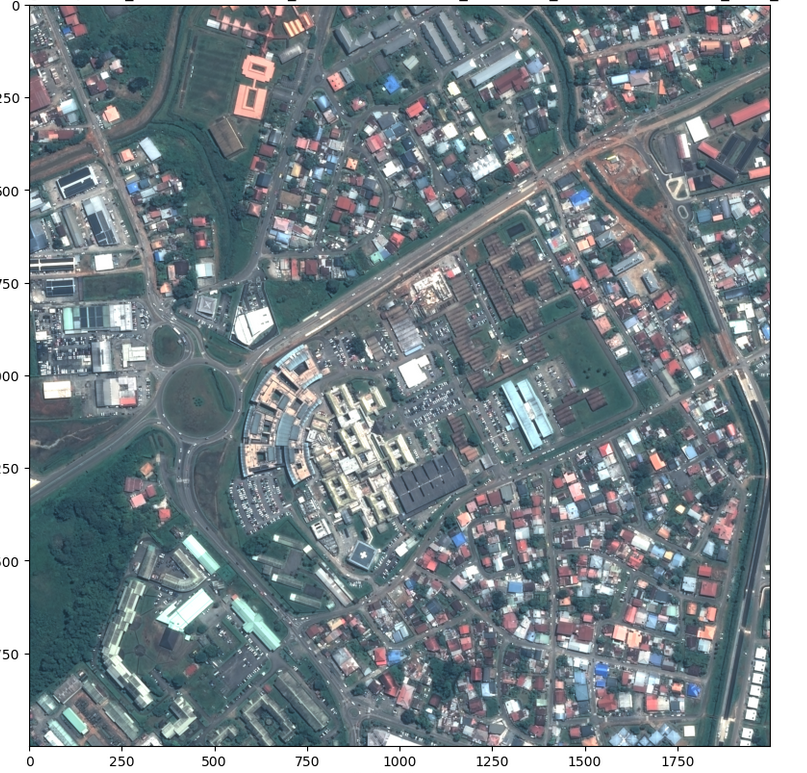
\includegraphics{figures/pleiade.png}

}

\caption{\label{fig-im-pleiade}Image Pléiades}

\end{figure}

\begin{itemize}
\tightlist
\item
  Résolution 50/70 cm, acquisitions fraîches mais coûteuses sur demandes
  \(\approx 1.5 \text{~~euros}/ km^{2}\)
\item
  En réalité résolution 1 bande 50 cm et réanchantillonnage des couleurs
  par dessus
\end{itemize}

\begin{figure}[H]

{\centering 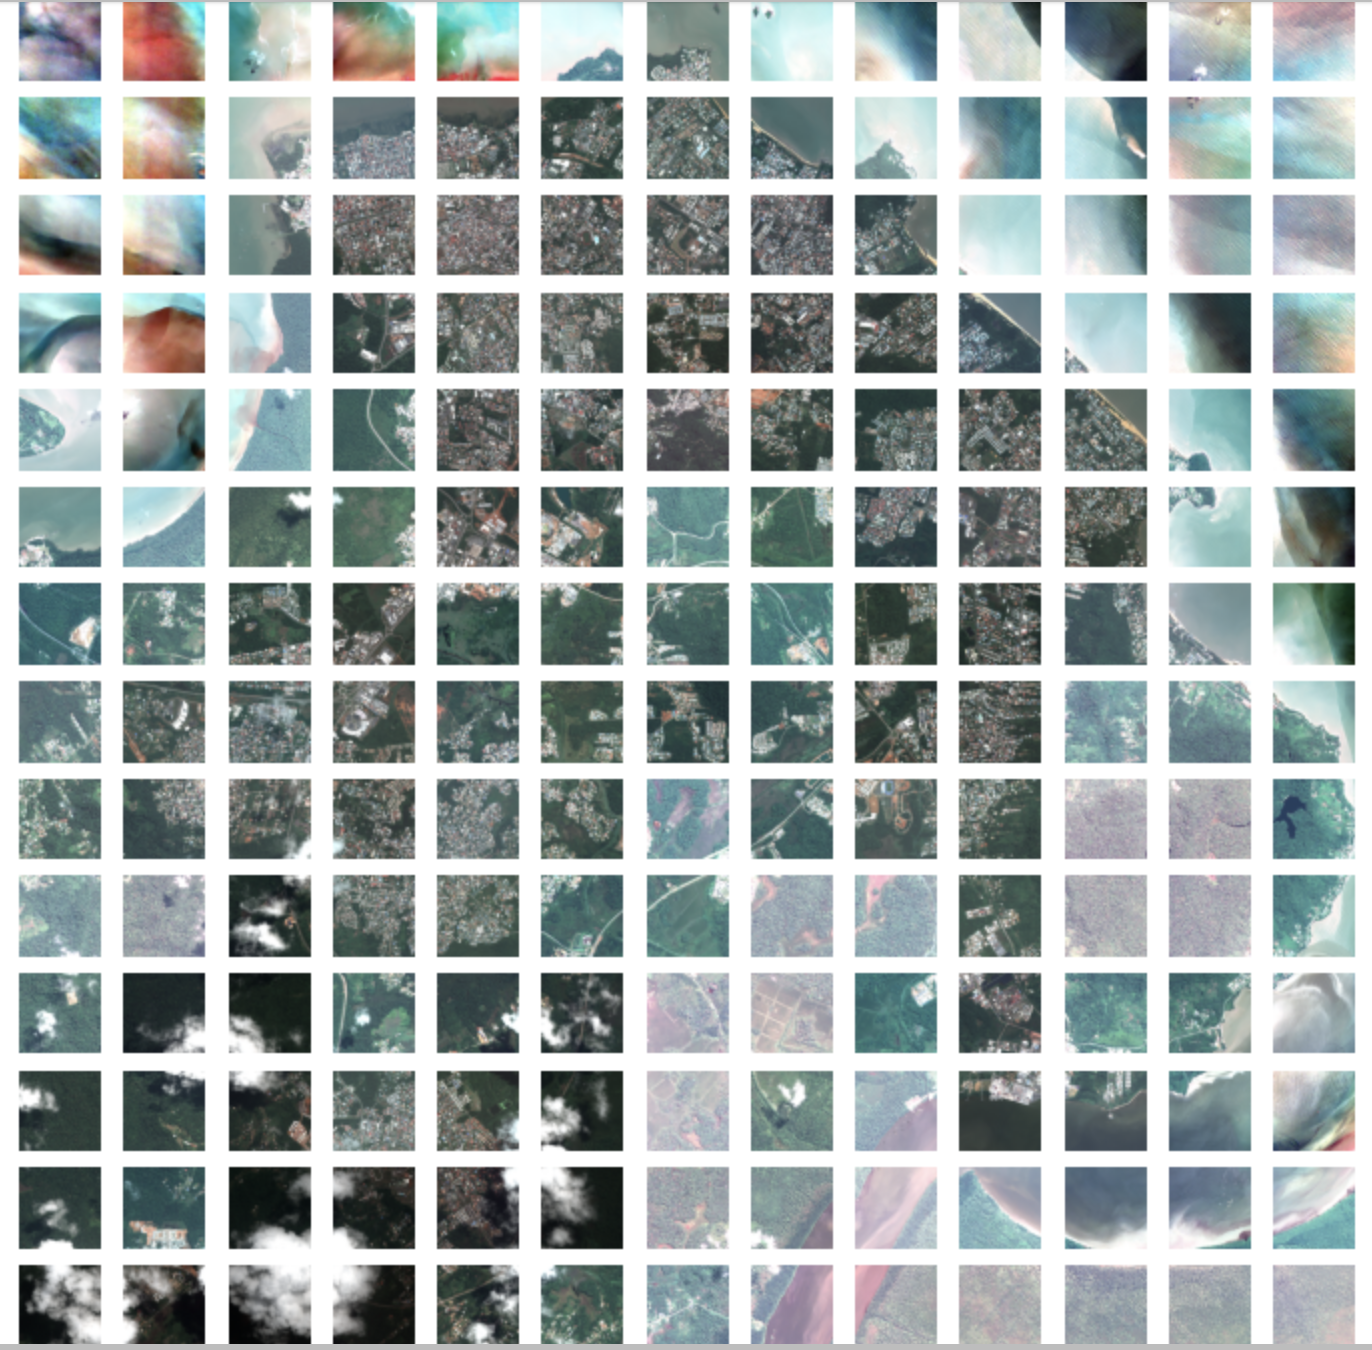
\includegraphics{figures/Grille_images.png}

}

\caption{\label{fig-pleiade-grid}Grille Pléiades Cayenne}

\end{figure}

\begin{itemize}
\tightlist
\item
  Les acquisitions peuvent être de plus ou moins bonnes qualité
  dépendant du moment de la prise de vue, on peut être amené à les
  refaire (nuage, ensoleillement), ça double les coûts.
\end{itemize}

Caractéristiques de la prise de vue pouvant nuire à la qualité de
l'image récupérée :

\begin{itemize}
\tightlist
\item
  La couverture nuageuse : trop de nuages \(\longrightarrow\) images non
  exploitables
\item
  Angle d'incidence : angle entre le satellite et la localisation
  considérée, si l'angle est trop élevé, trop de déformations dans la
  prise de vue
\end{itemize}

\begin{figure}[H]

{\centering 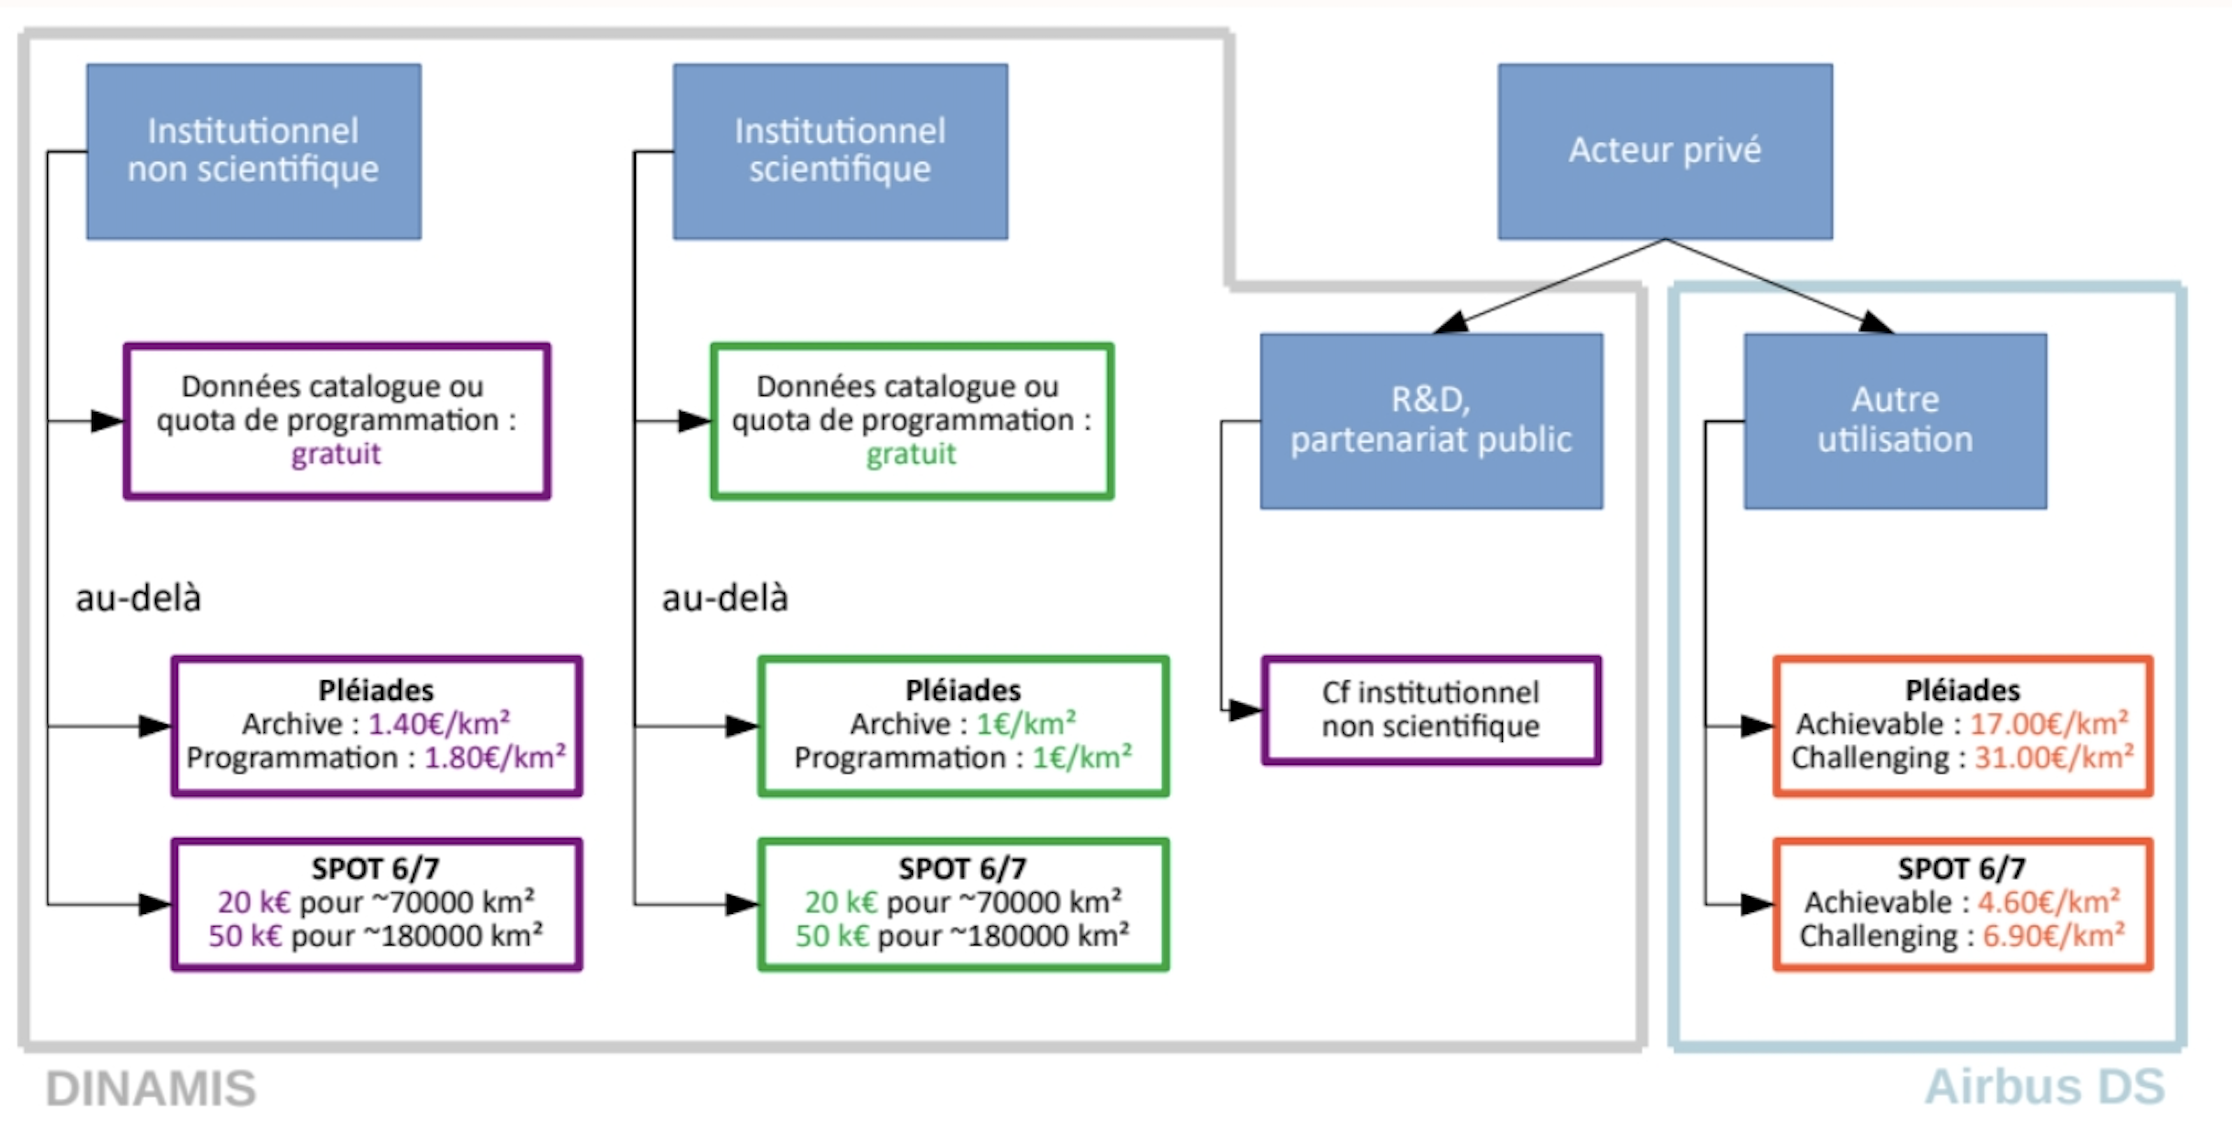
\includegraphics{figures/couts_pleiades.png}

}

\caption{\label{fig-pleiade-cost}Coûts Pléiades}

\end{figure}

\begin{figure}[H]

{\centering 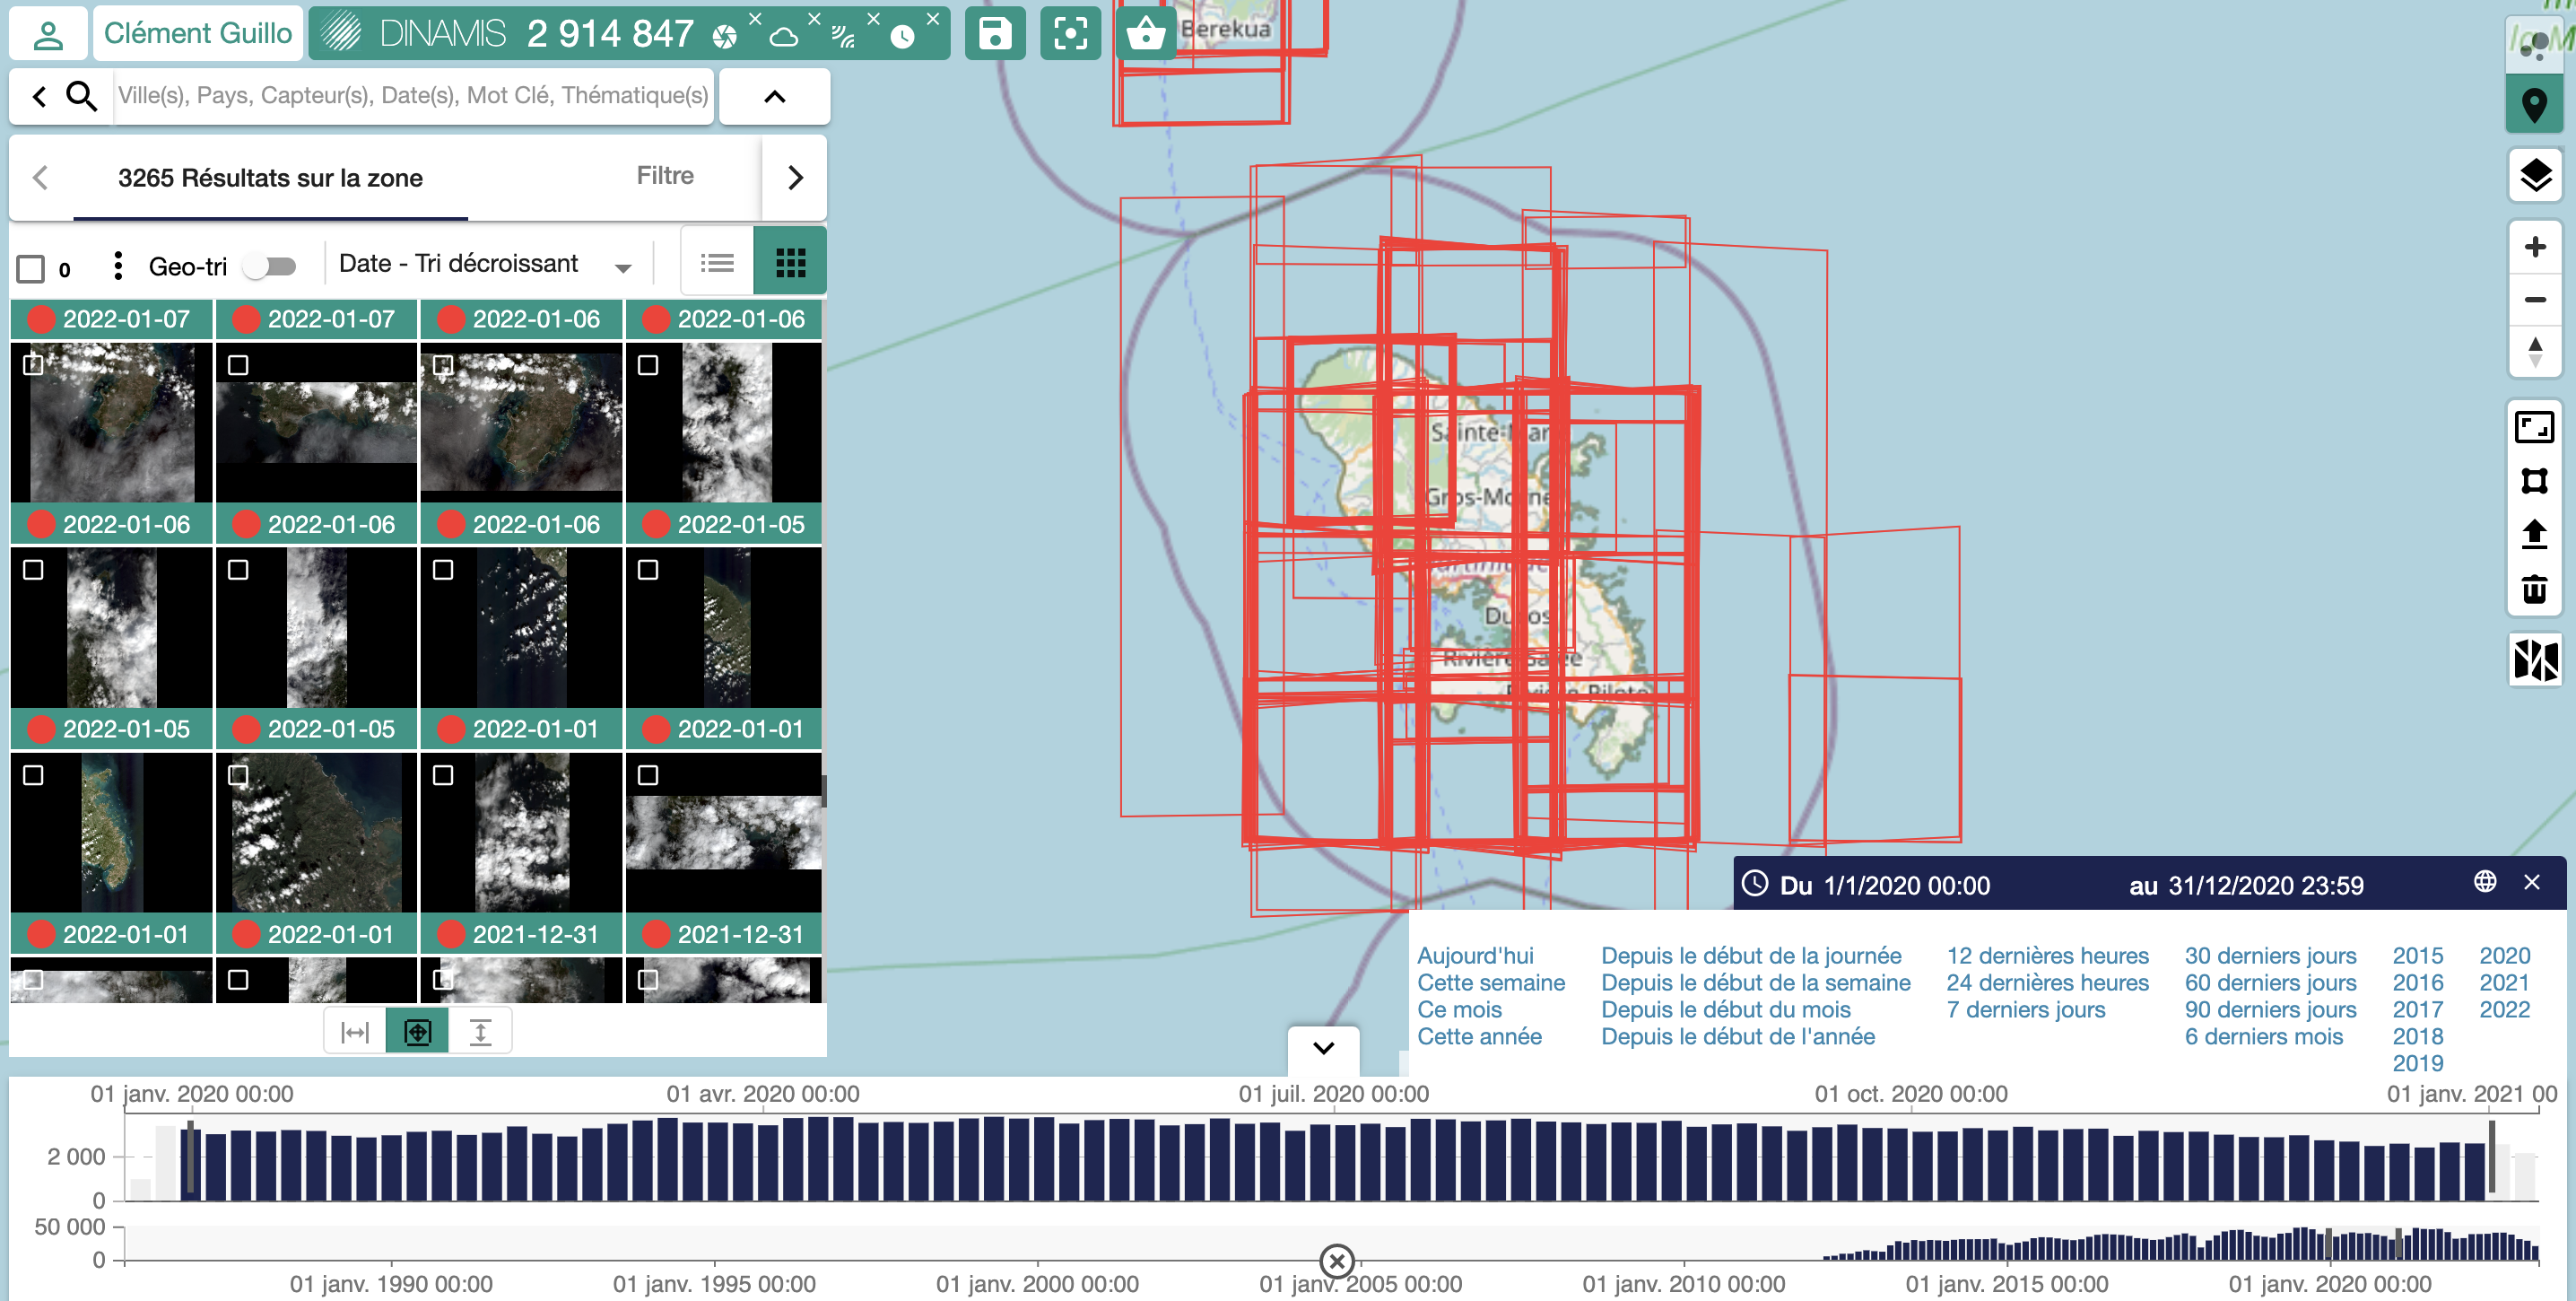
\includegraphics{figures/ElCatalogue.png}

}

\caption{\label{fig-catalogue}Catalogue Dinamis}

\end{figure}

\begin{longtable}[]{@{}ccc@{}}
\caption{Facturation des images hautes résolution
\(\approx 1.50 / km^2\).}\tabularnewline
\toprule\noalign{}
\textbf{Territoire} & \textbf{Superficie (\(km^2\))} & \textbf{Prix (en
euros)} \\
\midrule\noalign{}
\endfirsthead
\toprule\noalign{}
\textbf{Territoire} & \textbf{Superficie (\(km^2\))} & \textbf{Prix (en
euros)} \\
\midrule\noalign{}
\endhead
\bottomrule\noalign{}
\endlastfoot
Martinique & 1128 & 1692 \\
Guadeloupe & 1628 & 2442 \\
Réunion & 2512 & 3768 \\
Mayotte & 374 & 561 \\
Guyane & 83900 & 125850 \\
\end{longtable}

\begin{itemize}
\tightlist
\item
  Nécessite une approche en deux temps où on sélectionnerait au
  préalable grossièrement les zones que l'on veut vérifier (notamment en
  Guyane)
\item
  Quotas de gratuité pour les acteurs publics 4000 \(km^2\)
  monoscopiques.
\end{itemize}

\bookmarksetup{startatroot}

\hypertarget{references}{%
\chapter*{References}\label{references}}
\addcontentsline{toc}{chapter}{References}

\markboth{References}{References}

\hypertarget{refs}{}
\begin{CSLReferences}{1}{0}
\leavevmode\vadjust pre{\hypertarget{ref-duque_exploring_2017}{}}%
Duque, Juan, Jorge Patino, and Alejandro Betancourt. 2017. {``Exploring
the {Potential} of {Machine} {Learning} for {Automatic} {Slum}
{Identification} from {VHR} {Imagery}.''} \emph{Remote Sensing} 9 (9):
895. \url{https://doi.org/10.3390/rs9090895}.

\leavevmode\vadjust pre{\hypertarget{ref-mboga_detection_2017}{}}%
Mboga, Nicholus, Claudio Persello, John Bergado, and Alfred Stein. 2017.
{``Detection of {Informal} {Settlements} from {VHR} {Images} {Using}
{Convolutional} {Neural} {Networks}.''} \emph{Remote Sensing} 9 (11):
1106. \url{https://doi.org/10.3390/rs9111106}.

\end{CSLReferences}

\cleardoublepage
\phantomsection
\addcontentsline{toc}{part}{Appendices}
\appendix

\hypertarget{appendix-1}{%
\chapter{Appendix 1}\label{appendix-1}}



\end{document}
